\chapter{Introduction}

\section{Généralités sur les caches}

Jusqu'aux années 2000, la vitesse des processeurs a considérablement augmenté (loi de Moore) alors que le temps d'accès à la mémoire RAM (Random-Access Memory) est resté globalement le même. Pour permettre au processeur d'accèder plus rapidement à des éléments mémoire, des caches sont donc utilisés entre les processeurs et la RAM. Cela permet de hiérarchiser la mémoire, avec des éléments dont le temps d'accès est différent. Cette organisation hiérarchique de la mémoire présente plusieurs objectifs : \\
\begin{itemize}
\item permettre de contenir un nombre conséquent de données ;
\item être organisée de manière à être rapide ;
\item ne pas coûter trop cher.\\ 
\end{itemize}

Les caches permettent de stocker la mémoire utilisée récemment par le processeur, en se basant sur deux concepts: la localité spatiale et la localité temporelle. La localité temporelle stipule qu'une cellule mémoire accédée récemment sera très probablement utilisée dans un futur proche. La localité spatiale est l'idée que si l'on accède à une cellule mémoire $X$, la cellule mémoire $X+1$ a de grandes chances d'être utilisée. \\

Les mémoires de haut niveau -- les plus proches du processeur sont notées L1 -- sont généralement de petite taille. Leur coût est conséquent mais leur accès est très rapide. Il existe plusieurs niveaux de caches, $3$ dans la plupart des architectures récentes. Les L1 sont très rapides mais peuvent contenir peu de données (de l'ordre de la dizaine de Ko) alors que le L3 est plus lent mais contient beaucoup de données (de l'ordre du Mo). On peut résumer comme par la figure \ref{img:hierarchy} une hiérarchie mémoire classique.\\

\begin{figure}[!h]
\begin{center}
   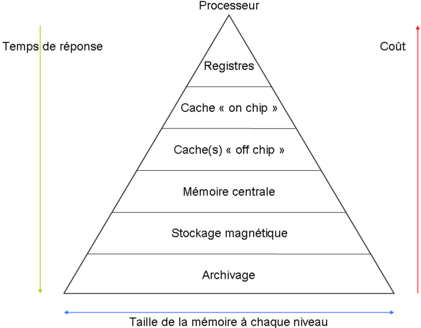
\includegraphics[scale=0.75]{hierarchy.png}
   \caption{\label{img:hierarchy} Hiérachie mémoire}
\end{center}
\end{figure}

==> Préciser source de l'image + légende\\

De cette manière, quand le processeur utilise une donnée qui est dans le cache, il fait un \textit{hit} : il n'a pas besoin de la charger à partir de la mémoire principale. Lorsque la donnée dont il a besoin n'est pas présente dans le cache, il fait un \textit{miss} et le coût d'accès à la donnée est beaucoup plus important. \\

Les données mémoire vont être lues via des \textit{load} et écrites via des \textit{store}. Lorsqu'une donnée est modifiée, il est nécessaire de propager les modifications jusqu'à la mémoire principale (c'est donc un \textit{store}), afin de garantir la cohérence du système. Une politique basique, le \textit{write-through}, serait de réécrire directement en mémoire après toute modification. Dans la suite de ce document, nous considérerons uniquement la politique \textit{write-back}, qui permet de retarder la réecriture tant que la donnée n'est pas lue pas une autre entité que celle qui l'a modifiée.

\section{Création d'un simulateur de caches}

Décrire ici notre projet. Partie copiée du cahier des charges éventuellement.

